\chapter{資料格式}

要理解瑲珩的資料格式,須要有一些基本的觀念。

要描述一個字符,最主要需要的資訊為其所組成的``部件''以及這些部件的``結合方式''。
以``曉''這個字為例,其可以分解成``日''和``堯'',而其結合方式為左右結合。

為方便說明,使用``運算''一術語來稱謂``結合方式''。
運算可以分兩種:一為內建的運算,一為``範本''。
所謂的範本,即為用來描述一種模式。
我們可以發現,很多字是具有類似的模式,
如:``品''、``晶''、``犇''都是三個相同的部件組成品字形。
又如:``贏''、``嬴''、``羸''都是類似結構。
範本就是指由內建運算所建立的模式。


此外,再以之前提到的``筆劃''來做說明。``曉''字可拆解成``日''和``堯''。
因此,要計算``曉''的筆劃數,可以由``日''的筆劃數加上``堯''的筆劃數。
然而,要計算``日''的筆劃數,則要一筆劃一筆劃地計數。
也就是,我們可以分成兩種部件,一種是可拆解的,另一種是不可拆解的。

對於合體字而言,其描述通常是與輸入法相獨立的。
如``曉''字可拆成``日''和``堯'',這點對任何輸入法都是一樣的。

而對於獨體字而言,其資訊則跟輸入法有關。
如:對計算筆劃而言,``日''為四劃,對倉頡而言,日的拆碼為日(a),
而對鄭碼而言,則為 k 。

在區分獨體字和合體字後。
上面所說,合體字的描述通常是與輸入法相獨立的,這點是不完全對的。
不同的輸入法有時也會對一些字有不同的拆解看法。
如``亘''這個字,在倉頡中的看法是由``一''、``日''、``一''所組成,
而在鄭碼中則視為``二''、``日''所組成。

縱合上述,將拆碼過程分為三步驟:
一、通用型拆碼,對大部分的輸入法都適用。將字拆成組件。
二、將組件拆成字根。
三、對組件編碼。



瑲珩定義了許多資料,資料位於 qhdata/ 。瑲珩資料檔分以幾種:
\begin{enumerate}
\item[一、]設定檔:位於 config/ 。說明一個輸入法或動態組字包含了哪些檔案。
\item[二、]結構檔:位於 main/ 及 main/component 及 component/ 。若同一個字符在不同目錄皆有定義,則以較後者。
其中 main/ 及 main/component 為所有輸入法共通的結構。 component/ 下則可以各輸入法有有不同。
\item[三、]範本檔:template/ 。定義範本。
\item[四、]字根描述檔:radix/。定義各字根。因各輸入法有不同的字根屬性,因此,沒有共通格式。
\item[五、]屬性檔:位於 frequency/ 。說明一個字符的屬性,目前只有字頻。
\item[六、]其它:如設定檔在 config/。
\end{enumerate}


結構檔的格式大略如下:
\listXML\begin{lstlisting}
	<瑲珩 版本號="0.3" 文件類型="組字">
		<字符集>
			<!--4E00-->
			<字符 名稱="一" 註記="U+4E00">
				<組字/>
			</字符>
			<字符 名稱="相" 註記="U+76F8">
				<組字 運算="範好">
					<字根 置換="木"/>
					<字根 置換="目"/>
				</組字>
			</字符>
		</字符集>
	</瑲珩>
\end{lstlisting}

其中,使用`<字符>'來說要為哪個字符定義結構。
意味著:`相'這個字是由`木'與`目'這兩個字以"範好"的方式所組成。
"範好"是由一個定義在範本中的運算,是指由兩個字左右組合。

範本檔示例如下:
\listXML\begin{lstlisting}
	<範本 名稱="範好">
		<參數列>
			<參數 名稱="女"/>
			<參數 名稱="子"/>
		</參數列>
		<組字結構>
			<組字 運算="鴻">
				<字根 置換="女"/>
				<字根 置換="子"/>
			</組字>
		</組字結構>
	</範本>
\end{lstlisting}


\section{運算與範本}
本計劃所定義及內建的運算有:
\begin{enumerate}
\item[一、]`龜':標示此部件無法被分解。如:木
\item[二、]`爲':此部件等同另一部件。如:釒即為金。
\item[三、]`龍':由多個部件結合成一個合體組件,沒有一定方向性。如:畞
\item[四、]`東':由多個部件結合成一個獨體組件。如:東。
\item[五、]`蚕':由多個部件呈現``縱向''的結合。如:想、臱。
\item[六、]`鴻':由多個部件呈現``橫向''的結合。如:相、湘。
\item[七、]`回':由多個部件呈現``包含''的結合。如:國、困。

\item[八、]`起':由兩個部件組合,呈現左下-右上的形式。如:趙、題。
\item[九、]`廖':由兩個部件組合,呈現左上-右下的形式。如:病、厄。
\item[十、]`載':由兩個部件組合,呈現右上-左下的形式。如:或,哉。
\item[十一、]`斗':由兩個部件組合,呈現右下-左上的形式。無例字。

\item[十二、]`同':由兩個部件組合,其中一個部件以三面包圍的方式圍住另一部件,開口向下。如:問、鳳。
\item[十三、]`函':由兩個部件組合,其中一個部件以三面包圍的方式圍住另一部件,開口向上。如:凶、函。
\item[十四、]`區':由兩個部件組合,其中一個部件以三面包圍的方式圍住另一部件,開口向右。如:匠、匿。
\item[十五、]`左':由兩個部件組合,其中一個部件以三面包圍的方式圍住另一部件,開口向左。無例字。

\item[十六、]`衍':由兩個部件組合,其中一個部件可拆成左右兩個小部件以夾住另一個部件。如:街、胤。
\item[十七、]`衷':由兩個部件組合,其中一個部件可拆成上下兩個小部件以夾住另一個部件。如:衷、裏。
\item[十八、]`粦':由三個部件組合,呈三角形排序。如:森。
\item[十九、]`瓥':由四個部件組合,呈田字形排序。如:歰、蠽。

\item[廿、]`畞':使用三個部件。如:畞。
\item[廿一、]`㘴':使用三個部件。如:㘴。
\item[廿二、]`幽':使用三個部件。如:豳。
\item[廿三、]`㒳':使用三個部件。如:繭。
\item[廿四、]`夾':使用三個部件。如:乖、爽。
\item[廿五、]`䜌':由三個部件以左右結合的方式組成,且左邊和右邊是相同部件,由中間先書寫。
\item[廿六、]`辦':由三個部件以左右結合的方式組成,且左邊和右邊是相同部件,由左邊先書寫。
\end{enumerate}

此外,對於漢字的最常見的幾種模式,在此列表如下:
\begin{enumerate}
\item[一、]`範好':兩個部件左右結合。
\item[二、]`範志':兩個部件上下結合。
\item[三、]`範湘':三個部件左右結合。
\item[四、]`範算':三個部件上下結合。
\item[五、]`範膷':四個部件左右結合。
\item[六、]`範纂':四個部件上下結合。
\item[七、]`範舝':五個部件上下結合。
\end{enumerate}

對於漢字的最常見的幾種重複模式,在此列表如下:
\begin{enumerate}
\item[一、]`範林':兩個相同的部件左右結合。
\item[二、]`範圭':兩個相同的部件上下結合。
\item[三、]`範㴇':三個相同的部件左右結合。
\item[四、]`範鑫':三個相同的部件成品字排列。
\item[五、]`範燚':四個相同部件成田字排列。
\end{enumerate}

一些字有類似的複雜結構,如:
\begin{enumerate}
\item[一、]`範贏':類似``贏''的結構,如:``嬴''、``羸''。
\item[二、]`範微':類似``微''的結構,如:``微''、``徽''。
\end{enumerate}



\section{動態組字}
與其他輸入法相同的是,動態組字使用一樣的結構描述。
只有在字根的部份訂定自己的格式。

其基本格式如下:
\listXML\begin{lstlisting}
	<瑲珩 版本號="0.3" 文件類型="字根" 輸入法="動態組字">
		<筆劃集>
		</筆劃集>
		<字根集>
		</字根集>
		<字符集>
		</字符集>
	</瑲珩>
\end{lstlisting}
其中,`<筆劃集>'預計用來定義常見筆劃,但目前並未使用。
其中,`<字根集>'預計用來定義常見字根。
其中,`<字符集>'預計用來定義常見字符。

這裡的字符指的是可以用來作用運算的部件。
這裡的字根指的是可以用來構成字符的部件。

字根示例如下
\listXML\begin{lstlisting}
	<筆劃集>
		<字根 名稱="$口" 註記="U+53E3">
			<筆劃組 名稱="$口%1">
				<幾何 範圍="0000FFFF"/>
				<筆劃 範圍="0000FFFF" 名稱="$口#1" 資訊表示式="(豎)00002E34,00012EC9"/>
				<筆劃 範圍="0000FFFF" 名稱="$口#2" 資訊表示式="(橫折)00002E34,0001CE34,0001CEC9"/>
				<筆劃 範圍="0000FFFF" 名稱="$口#3" 資訊表示式="(橫)00002EC3,0001CEC3"/>
			</筆劃組>
		</字根>
	</筆劃集>
\end{lstlisting}


字符示例如下:
\listXML\begin{lstlisting}
	<字符集>
		<字符 名稱="古" 註記="U+53E4">
			<編碼資訊>
				<編碼>
					<筆劃組>
						<幾何 範圍="0000FFFF"/>
						<筆劃 範圍="0000FFFF" 資訊表示式="(橫)00001048,0001DF48"/>
						<筆劃 範圍="0000FFFF" 資訊表示式="(豎)00007519,0001758A"/>
						<筆劃 範圍="0080FFFF" 資訊表示式="$口%1"/>
					</筆劃組>
				</編碼>
		</編碼資訊>
	</字符>
	</字符集>
\end{lstlisting}

\section{筆劃}
一個筆劃是以類似"(橫)00001048,0001DF48"的方式,其中的"(橫)"用來說明這個筆劃的類型。
\begin{enumerate}
\item[一、]點。示例:`主'的第一筆。
\item[二、]長頓點。示例:`下'的最後一筆。

\item[三、]橫。示例:一。
\item[四、]橫鉤。示例:
\item[五、]橫折。示例:
\item[六、]橫折橫。示例:
\item[七、]橫折鉤。示例:
\item[八、]橫撇。示例:
\item[九、]橫曲鉤。示例:
\item[十、]橫撇橫折鉤。示例:
\item[十一、]橫斜鉤。示例:
\item[十二、]橫折橫折。示例:

\item[十三、]豎。示例:`中'的最後一筆。
\item[十四、]豎折。示例:
\item[十五、]豎挑。示例:
\item[十六、]豎橫折。示例:
\item[十七、]豎橫折鉤。示例:
\item[十八、]豎曲鉤。示例:
\item[十九、]豎鉤。示例:
\item[廿、]臥鉤。示例:`心'的第二筆。
\item[廿一、]斜鉤。示例:`戈'的第二筆。
\item[廿二、]彎鉤。示例:`手'的最後一筆。

\item[廿三、]撇。示例:
\item[廿四、]撇頓點。示例:
\item[廿五、]撇橫。示例:
\item[廿六、]撇挑。示例:
\item[廿七、]撇折。示例:
\item[廿八、]豎撇。示例:
\item[廿九、]挑。示例:
\item[卅、]挑折。示例:
\item[卅一、]捺。示例:

\item[卅二、]挑捺。示例:`乀'。
\item[卅三、]橫捺。示例:`乁'。
\item[卅四、]圓。示例:`㔔'的最後一筆。
\end{enumerate}

點得描述則為 `AAAAXXYY' 。其中,AAAA表示運算。XX及YY為十六進位,分別表示(x,y)。
AAAA 為 0000, 0001, 0002 。0000為起始,0001為畫到,0002則為曲線的輔助點。


\subsection{空間描述}
一個字符是由許多部件構成,而彼此所佔空間的比例將影響美觀。
因此空間分配很重要。

有些為較複雜的結構組合,如左下-右上。
如:床=广+木

\begin{center}
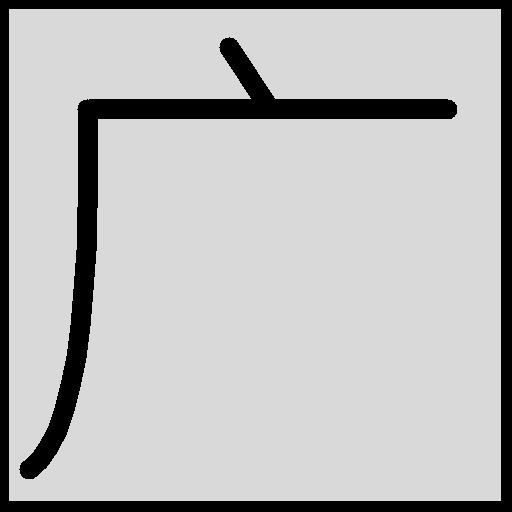
\includegraphics[scale=0.25]{picture/yan.png}
\end{center}

\begin{center}
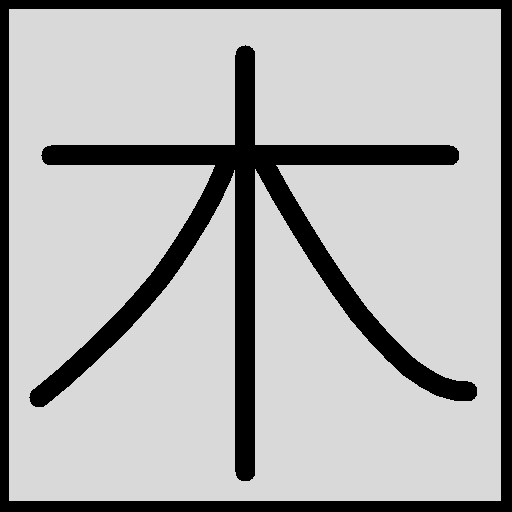
\includegraphics[scale=0.25]{picture/mu.png}
\end{center}

而兩者組合後的結果如下:
\begin{center}
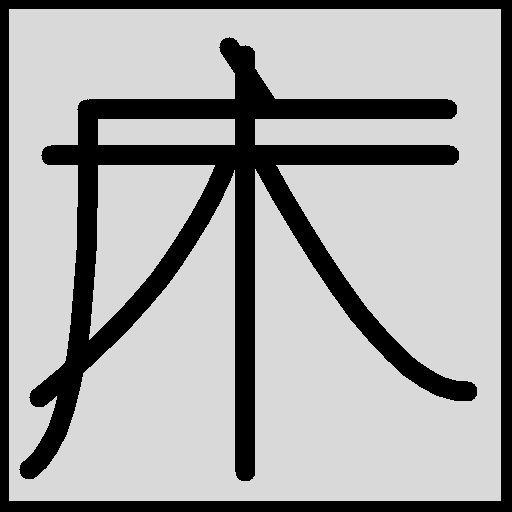
\includegraphics[scale=0.25]{picture/chuang_bad.png}
\end{center}

於是,在描述字形時,同時描述一些空間描述。
\begin{center}
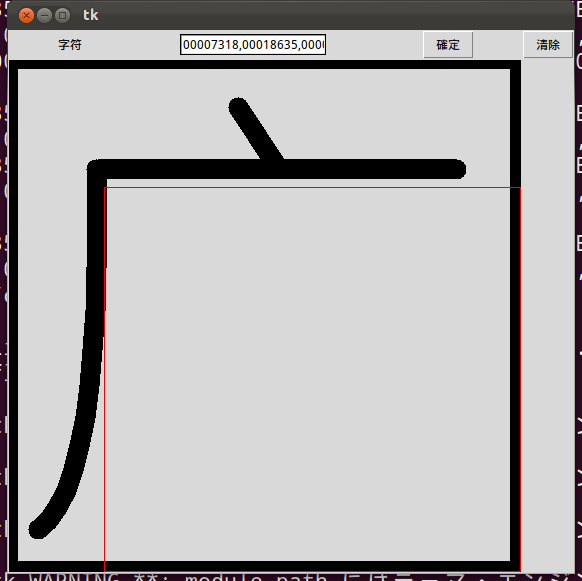
\includegraphics[scale=0.25]{picture/yan_extend.png}
\end{center}
紅色框的部份則是放置其他字符所能使用的範圍。

\listXML\begin{lstlisting}
	<字符 名稱="广" 註記="U+5E7F">
		<編碼資訊>
			<編碼>
				<補充範圍 名稱="廖">
					<幾何 範圍="3040FFFF"/>
				</補充範圍>
				<筆劃組>
					<幾何 範圍="0000FFFF"/>
					<筆劃 範圍="0000FFFF" 資訊表示式="(點)00007318,00018635"/>
					<筆劃 範圍="0000FFFF" 資訊表示式="(橫)00002D37,0001E037"/>
					<筆劃 範圍="0000FFFF" 資訊表示式="(豎撇)00002C37,00022FD5,00010FEB"/>
				</筆劃組>
			</編碼>
		</編碼資訊>
	</字符>
\end{lstlisting}

兩者組合後的結果如下:
\begin{center}
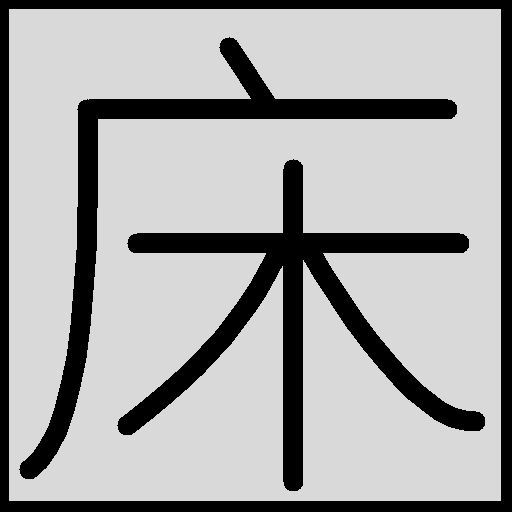
\includegraphics[scale=0.25]{picture/chuang_good.png}
\end{center}

